\chapter{Setup}
\label{chapterlabel2}
% \section{Overview}
%As mentioned previously,  this project looks to implement convolutional networks for video classification, particularly looking at action labelled data.
% explain convultional netweorks with pooling layer

% with the future aim of exploring with emotion classification using image and video data. Something that has been explored in papers such as \cite{SUN201836}
% explain f what a convutional neural network is here, talk about Alexnet
% In order to get familiar with building neural networks, the first task involved  then understanding the structure and looking atthe performance of pretrained models CNN models readily available.



\section{Environment and Software}
% todo explain the clusters better
%what is pip
Since the project required TensorFlow and the Keras API with python programming language, python 3.6 was used as it is the newer and more compatible python version from the legacy soon to be deprecated python 2.7.
The initial coding environment set up was done using Anaconda which is  an open-source distribution for python and python libraries which are typically used for scientific computing. Anaconda also provides distribution of other statistical tools such as R-studio which is used for the R programming language.
Another benefit of Anaconda is that it allows for multiple python environments and easy download of libraries. It has a very friendly user graphical interface as well as a command-line interface.
%todo pip and reference
Pip which is the python specific library management tool, was also used to download some TensorFlow libraries which were not available in Anaconda.

TensorFlow comes in two distribution the first being the Graphics processing unit (GPU) enabled distribution with uses the GPU first by default to speed up specific processes before it uses the (Central processing unit ) CPU.
The second distribution, which is also the default distribution runs on the CPU only.
The project initially began on a laptop with no GPU capacity. Hence the TensorFlow default package was installed.

The impressive quality of TensorFlow, is its use of a dataflow graph. In the TensorFlow dataflow graph, the nodes represent units of computation, and the edges represent the input data or the output data of the computation. This dataflow graph allows for benefits such as the use of parallel computing for model training ad running, distributed execution through the use of explicit edges which allows for partitioning across multiple devices. The dataflow graph also improves compilation and generates faster code by allowing TensorFlow's XLA compiler to use dataflow graph information. The dataflow graph is also language-independent, allowing for portability between language.
TensorFlow comes with a keras API within its libraries, this version of Keras supports the use of the dataflow graph unlike the readily available Keras library.  As TensorFlow provides the Keras API,  there was no need to download keras separately.
The project also initially began in a jupyter notebook environment which is an open-sourced web-based interactive development environment used for a multitude of scientific research. An Empirical Study on Jupyter notebook as a tool for scientific research has also been taken as seen in \citep{Randles_2017}. While on jupyter notebook, TensorFlow was running in eager mode.  Eager mode is a programming environment provided by TensorFlow which evaluates operations from the dataflow graph immediately. It does this by not building computational graphs, hence allowing concrete values to be returned instead of constructing a graph to run later, making debugging easier in such an interactive environment like jupyter notebook.
Once familiar with the working of the Tensorflow environment, The models were then transferred into python scripts.

% Rather building models from scracth the TensorFlow package and keras  packages where used to construct the models and access the pre-trained models.

\section{Datasets}
TensorFlow also provides readily available pre-processed data sets for easy use. These datasets are available using the TensorFlow dataset library. The TensorFlow dataset is a library that exposes publicly available datasets as numpy arrays, TensorFlow dataset object or tensors. The datasets range from images to audio to text datasets. Some popular datasets include MNIST database of handwritten digits \citep{6296535}. 
This project used the UCF101 dataset provided by TensorFlow dataset library. The UCF101 dataset is an action recognition dataset of realistic action videos, collected from YouTube, having 101 action categories \cite{soomro2012ucf101}. It contains about 13320 videos for the 101 action categories. The videos in the 101 action categories are grouped into 25 groups, where each group can consist of 4-7 videos of an action. The videos from the same group may share some common features, such as similar background, similar viewpoint, etc.
The action categories can be divided into five types which include Human-Object Interaction, Body-Motion Only, Human-Human Interaction , Playing Musical Instruments and Sports.
Tensorflow also provides a train test split of the data where the number of training examples is 9537, and the number of test examples is 3783.
It also provides the functionality to take a custom spilt of the data and reduce the number of videos used for training. Each clip contains multiple frames of 256x256x3. The frames were taken at a  rate of 25 fps. The clips range in length from about 1.06 seconds to  71.04 seconds.
%todo crosscheck how youtube-8m download works%
This UCF101 dataset is also used in \citep{KarpathyCVPR14} to train models based off pre-trained models trained with the larger data set of sports-1M.
The  sports-1M dataset, which consists of over one million YouTube videos belonging to about 487 classes of sports which was used \citep{KarpathyCVPR14}. Could not be used because although it is readily available on youtube with most of the links supplied in it's GitHub repository.  This is because downloading a dataset of that magnitude proposes a challenge with the memory needed to store the dataset — also the time required in downloading this large dataset. Such a large dataset can also lead to extremely long training time. There is also the challenge of copyright as no clear instructions on copyright was set for all the applicable videos from Youtube. Hence because of this and the time constraints with the project, the smaller UCF101 dataset was used to recreate the models. It is also important to note that the sports-1M is also available as part Youtube-8M dataset. And although there is an API available to download videos from the Youtube-8M as TensorFlow Record file, the sports-1M dataset cannot be easily specified for download from the Youtube-8M as it does not allow for access to specific videos. Which would have been an excellent addition because the sport-1M dataset GitHub page provides the list of videos included in the sport-1M dataset split into training and test datasets.

% might be worth summaring the dataset used in karpathy's paper

\section{Computation}
Most of the models had a long-running time when ran in the jupyter notebook environment, So it needed to be run over a long period of time with a capable computer infrastructure.  Then UCL cluster infrastructure was then used for running the models. The scripts were initially run in the cluster log in the terminal. Then they were running for a short time, in the interactive session, which allows the setup of the required memory and processing power needed to run. This was used to gauge the right setup by comparing the speed per each epoch and step for different configurations.  Once decided on the setup, such as the RAM required and the number of GPUs required. The clock time, which is how long the model will run for was decided. Then the batch jobs were set up to run the models from the python scripts.


\section{Architectures}

In \citep{KarpathyCVPR14} paper on Large-scale Video Classification with Convolutional Neural Networks \citep{KarpathyCVPR14}, it discusses various models and explores approaches for fusing information over temporal dimension through the convolutional network and compares their performance. Using the UCF101 dataset and TensorFlow, this project will also explore recreating these models and apply newer techniques for optimization. The models which will be implemented are listed below. The structures of these models can be also be seen in figure \ref{fig:k_models} taken from \citep{KarpathyCVPR14}
\begin{itemize}
    \item Single Frame: is loosely based on the Alexnet model \cite{NIPS2012_4824}, which was the winning model of the ImageNet challenge in 2012. Alexnet model takes in an input image of $224 \times 224 \times 3$, using the shorthand notation as described in \citep{KarpathyCVPR14}, the full architecture is $C(96, 11, 4)-N-P-C(256, 5, 1)-N-P-C(384, 3, 1)-C(384, 3, 1)-C(256, 3, 1)-P-F C(4096)-F C(4096)$, where $C(d, f, s)$, is a convolutional layer with d filters of spatial size $ f × f$, with a stride of $s$,  $FC(n)$ is a fully connected layer with n nodes, $N$ is local response normalization layer and P is the pooling layer. The single frame model from \cite{KarpathyCVPR14} follows the following architecture  $C(96, 11, 3)-N-P-C(256, 5, 1)-N-P-C(384, 3, 1)-C(384, 3, 1)-C(256, 3, 1)-P-F C(4096)-FC(4096)$ with the exception that it takes in an image of size $ 170 \times 170 \times 3$. The single frame also uses a max-pooling of a non-overlapping with size $2 \times 2$ rather than overlapping pooling of size $3x3$ and stride $2$ used in the Alexnet. This is an interesting difference that might have an effect on performance as the Alexnet paper suggest that generally, they observed during training that models with overlapping pooling found it slightly more difficult to overfit.
    \item Early Fusion - This combines information across an entire time window immediately on the pixel level hence making the input size that of $11 \times 11 \times 3 \times T$ pixels, where T was 10 which is also the number of frames covered. The change in input shape also required a change to the first convolutional layer to use a filter size of $10 \times 11 \times 11$.
    \item Late Fusion: This uses two single frame networks that have input frames that are about 15 frames apart. The single frame networks are combined at the fully connected layers.
    \item Slow Fusion: This is a mix of both late and early fusion. It slowly combing the temporal information over at each convolutional layer. The input is a set of 10 frames from a clip. The first convolution layer now consists of 4 parallel layers that each take in 4 frames out of the initial 10 frames, The second convolutional layer consist of two parallel layers that combine the two outputs from the first while the third layer combines the output from the second layer
\end{itemize}

\begin{figure}
    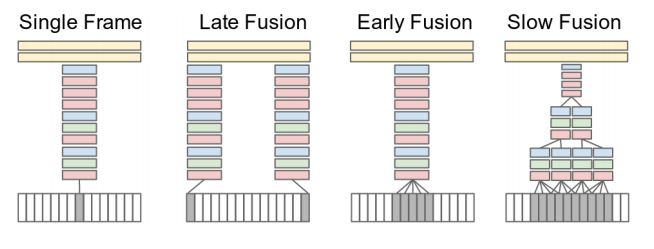
\includegraphics[width=\linewidth]{K_models.JPG}
    \caption{\citep{KarpathyCVPR14} Explored approaches for fusing information over temporal dimension through the network.  The Red, Green and Blue boxes indicate convolutional, normalization and pooling layers respectively}
    \label{fig:k_models}
\end{figure}

There is a wide range of a pre-trained convolution neural networks architectures particularly models for image classification trained on ImageNet dataset available via the Keras API.  A few of these where also explored as listed below.
\begin{itemize}
    \item VGG19: as described in \citep{simonyan2014deep}, is quite a standard convolutional neural network architecture that consists of a $3 \times3$  filters with a stride 2, followed by a $2\times2$ max-pool filter with a stride of 2.
    \item MobileNetV2: is a model created for mobile vision application a. MobileNetV2 as discussed in \cite{Sandler_2018} improves on its predecessor MobileNetV1 as discussed in \citep{howard2017mobilenets}.  MobileNetV1 uses a depthwise separable convolution as efficient building blocks while MobileNetV2 introduces a linear bottleneck between the layers and a shortcut connections between the bottlenecks.
    \item Inception: this convolutional neural network architecture as discussed in \citep{Szegedy_2016} is made up of inception blocks which evaluate multiple, multiple pooling layers of different dimensions then concatenate the results.
    \item ResNet: this architecture \citep{He_2016} is made up of residual blocks. These residual blocks are a set of two layers that rather than going through the standard path of going from one activation layer to the next, passes the linear equation output to the next layer activation function to arrive at the activation value for the next layer. This is believed to have the benefit of helping with vanishing and exploding gradients to improve performance as the neural network gets deeper.
\end{itemize}


\section{Assumptions}
Some assumptions were made on the implementation of the models such as the starting frame for the model inputs.  This was because it was not explicitly made clear in the text in \citep{KarpathyCVPR14}. Although one could argue that in figure \ref{fig:k_models}, the 7th frame from the start point of the model was used.  However, initially, all model implementation, the first frame was selected as the starting frame. For example, this means with the single frame implementation, the first frame of the clip was the input frame.  The seemed like a modest assumption because as discussed in \citep{soomro2012ucf101} which discussing the UCF101 dataset, the videos have a huge variation in length hence to avoid any issues such as selecting a frame in a position that does not exist.

In \citep{KarpathyCVPR14}, they talk about using downpour stochastic gradient descent to optimize the models across a computing cluster. They used about 10 to 50 replicas for each model; they further split every model across 4 to 32 partitions. They also use mini-batches of 32 examples, momentum of 0.9, weight decay of 0.0005 and a  learning rates of $1e^{-3}$, which was further reduced by hand whenever the validation error stops improving.  However, for this project, a more simplified optimization was used which was inspired from \citep{KarpathyCVPR14}. The optimization uses initially for all models was a stochastic gradient descent with mini-batches of 32 examples, momentum of 0.9, weight decay of 0.0005 and a static learning rates of $1e^{-3}$.

\citep{KarpathyCVPR14} also does not specify the loss function used; however, since there was a reasonably large number of categories for the UCF101 dataset sparse categorical cross-entropy seemed like the best option. This was also because unlike its counterpart categorical cross-entropy which is also used for multi-classification; sparse categorical cross-entropy requires a one-hot encoded. 

A standard accuracy performance metric was also used when  training and validating the model as none where specifically specified in \citep{KarpathyCVPR14}

%and the first frame with is extended for the other models such as the late fusion and slow fusion models%
